\documentclass[openany,12pt,a4paper]{report}
\usepackage{subfiles}
\usepackage[numberedsection]{glossaries}
\usepackage[]{graphicx}
\usepackage{float}
\usepackage{multirow}
\graphicspath{{./img/}{./../img/}}
\usepackage{../StileDoc}
\title{Manuale Sviluppatore}
\author{}

%Ultima versione documento
\newcommand{\versione}{1.0.0}

% Stile per il glossario
\newglossarystyle{glossaryStyle}{
	\setglossarystyle{altlistgroup}
	\renewcommand*{\glsgroupheading}[1]{
		% Tolgo la numerazione per l'indice
		\setcounter{secnumdepth}{0}
		\section{##1}
		\vspace*{-\baselineskip}
		% Solo per fare un po' di spazio tra la lettera e le voci
		\item\makebox[\linewidth]{\hspace*{2cm}}
	}
}

\glsaddall

\makeglossaries

%Term definitions
\newglossaryentry{Speect}{name=Speect, description={Libreria di Text-To-Speech di riferimento per il progetto DeSpeect}}
\newglossaryentry{GCC}{name=GCC, description={Compilatore C++ di riferimento per il progetto DeSpeect}}
\newglossaryentry{Qt Creator}{name={Qt Creator}, description={Ambiente di sviluppo integrato (IDE) multipiattaforma per creare applicazioni C ++ e QML}}
\newglossaryentry{GitHub}{name=GitHub, description={Servizio di versionamento per progetti software}}
\newglossaryentry{Qt}{name=Qt, description={Libreria multipiattaforma per lo sviluppo di programmi con interfaccia grafica tramite l'uso di widget}}
\newglossaryentry{IDE}{name=IDE, description={un ambiente di sviluppo integrato (in lingua inglese integrated development environment ovvero IDE) è un software che, in fase di programmazione, aiuta i programmatori nello sviluppo del codice sorgente di un programma}}
\newglossaryentry{utterance}{name={Utterance}, description={La più piccola unità del discorso, una parte di esso che inizia e termina con una pausa chiara}}
\newglossaryentry{relation}{name={Relation}, description={Rappresenta una struttura come una parola, sillaba, fonema o anche un obiettivo di durata e gli item sono il contenuto di questa struttura.}}
\newglossaryentry{plug-in}{name={Plug-in}, description={Un programma non autonomo che interagisce con un altro programma per ampliarne o estenderne le funzionalità originarie}}
\newglossaryentry{framework}{name={Framework}, description={Piattaforma che funge da strato intermedio tra un sistema operativo e il software che lo utilizza.}}


\begin{document}
	
	\makeatletter
	\begin{titlepage}
		\setlength{\headsep}{0pt}  
		\begin{center}
			
\includegraphics[width=0.5\linewidth]{img/logo.png}\\[1em]
			{\huge \bfseries  \@title }\\[10ex]
			\textbf{\Large Informazioni Documento} \\[2em]
			\bgroup
			\def\arraystretch{1.5}
			\begin{tabular}{l|l}
				\textbf{Versione} & \versione{} \\
				\textbf{Data approvazione} & 10 Marzo 2018 \\
				\textbf{Responsabile} & Marco Focchiatti\\
				\textbf{Redattori} &  Manfredi Smaniotto, Marco Focchiatti,\\
				& Cristiano Tessarolo, Giulio Rossetti \\
				\textbf{Verificatori} & Manfredi Smaniotto, Marco Focchiatti \\
				\textbf{Distribuzione} & Prof. Tullio Vardanega \\
				& Prof. Riccardo Cardin \\
				& Mivoq S.R.L. \\
				& Gruppo Graphite \\
				\textbf{Uso} & Esterno \\
				\textbf{Recapito} & graphite.swe@gmail.com \\
			\end{tabular}
			\egroup
		\end{center}
	\end{titlepage}
	\makeatother
	
	\thispagestyle{empty}
	\newpage
	
	%REGISTRO DELLE MODIFICHE
	
	\chapter*{Registro delle modifiche}
	\setlength\LTleft{-22mm}
	\begin{longtable}{|p{20mm}|p{20mm}|p{40mm}|p{30mm}|p{50mm}|}
		\hline
		\textbf{Versione} & \textbf{Data} & \textbf{Autore} & \textbf{Ruolo} & \textbf{Descrizione} \\
		
		\hline 1.0.0 & 2018-04-15 &  & Responsabile & Approvazione \\
		\hline 0.2.0 & 2018-04-15 & - & Verificatore & Verifica da §5 a §8 e appendici \\
		\hline 0.1.4 & 2018-04-14 & - & Amministratore & Stesura appendici \\
		\hline 0.1.3 & 2018-04-13 & - & Amministratore & Stesura §8 \\
		\hline 0.1.2 & 2018-04-12 & - & Progettista & Stesura §7 §3 \\		
		\hline 0.1.1 & 2018-04-12 & - & Progettista & Stesura §5 - §6 \\
		\hline 0.1.0 & 2018-04-11 & - & Verificatore & Verifica da §1 a §4 \\
		\hline 0.0.5 & 2018-04-08 & - & Amministratore & Stesura §4 \\	
		\hline 0.0.4 & 2018-04-08 & - & Amministratore & Stesura §3 \\
		\hline 0.0.3 & 2018-04-07 & - & Amministratore & Stesura §2 \\
		\hline 0.0.2 & 2018-04-06 & - & Amministratore & Stesura §1 \\
		\hline 0.0.1 & 2018-04-05 & - & Amministratore & Creata struttura documento \\
		\hline
		
	\end{longtable}
	
	
	% INDICE
	\tableofcontents
	
	% INTRODUZIONE
	
	\chapter{Introduzione}
	
	\section{Scopo del documento}
	
	Il documento ha la finalità di illustrare a coloro che volessero interfacciarsi con l’applicazione
	\textit{"DeSpeect: un'interfaccia grafica per Speect"} le modalità di installazione e di utilizzo, i requisiti necessari per poterlo utilizzare, le librerie e i \glossario{framework}{framework} esterni utilizzati per lo sviluppo dell’applicazione,
	oltre alla sua architettura, così da aiutare
	nella ricerca o eventuale estensione delle sue funzionalità. Nonostante la versione attuale rappresenti una prima bozza del documento, una volta concluso esso rappresenterà un riferimento completo per l’utilizzo del prodotto da parte di uno sviluppatore.
	
	\section{Scopo del prodotto}
	
	Lo scopo del progetto è la realizzazione di un’interfaccia grafica per \glossario{Speect}{Speect} [Meraka Institute(2008-2013)], una libreria per la creazione di sistemi di sintesi vocale, che agevoli l’ispezione del suo stato interno durante il funzionamento e la scrittura di test per le sue funzionalità.
	
	\section{Informazioni utili}
	
	La stesura di questo documento assume come utente target del prodotto un programmatore esperto nell'utilizzo di \textit{Speect} e dei linguaggi di programmazione C e C++.
	Per completezza, viene riportato in appendice D un glossario comprensivo di termini tecnici o riguardanti particolari funzionalità di \textit{DeSpeect}. Per identificare i termini
	presenti nel glossario, la loro prima occorrenza all’interno del documento è riportata in corsivo e
	marcata con una G al pedice.
	
	\section{Riferimenti informativi}
	
	\begin{itemize}
		\item \textbf{Documentazione Speect:} \\
		\url{http://speect.sourceforge.net/contents.html};
		\subitem Documentazione ufficiale della libreria di \textit{Text-To-Speech} di riferimento per il progetto.
		
		\item \textbf{Documentazione Qt:} \\
		\url{http://doc.qt.io/};
		\subitem Documentazione ufficiale del framework utilizzato per lo sviluppo dell'interfaccia grafica.
		
		\item \textbf{Documentazione CMAKE:} \\
		\url{https://cmake.org/documentation/}.
		\subitem Documentazione ufficiale del framework utilizzato per la build del prodotto. 
	\end{itemize}

	\chapter{Requisiti di sistema}
	
	L'installazione ed esecuzione del software DeSpeect richiede i seguenti prerequisiti:
	
	\begin{itemize}
		\item Sistema operativo Unix / Unix-like (il software è stato testato solo per piattaforma Ubuntu 16.04 LTS)
			\subitem \url{https://www.ubuntu.com/download/desktop}
		\item CMake (versione minima 2.8)
			\subitem \url{https://cmake.org/download/}
		\item Compilatore ANSI C/ISO C90 \glossario{GCC}{GCC} (versione minima 5.0)
			\subitem \url{https://gcc.gnu.org/install/binaries.html}
		\item \glossario{Qt}{Qt} 5.9.0
			\subitem \url{https://www.qt.io/download}
		\item Git
			\subitem \url{https://git-scm.com/} 
		\item Curl 
			\subitem \url{https://curl.haxx.se/}
		\item Swig 
			\subitem \url{http://www.swig.org/}
		\item libxml2-dev
			\subitem \url{https://packages.debian.org/stretch/libxml2-dev} 
		\item python-dev
			\subitem \url{https://pypi.python.org/pypi/dev/0.4.0}
	\end{itemize}

	\chapter{Tecnologie impiegate}
	
	Vengono di seguito illustrate le tecnologie impiegate dal software DeSpeect e nella verifica e monitoraggio del suo codice.
	
	\section{Tecnologie utilizzate da DeSpeect}
	
	\subsection{Libreria di riferimento}
	Speect è un sistema di \textit{Text To Speech} (TTS) multilingua. Esso offre un sistema TTS completo (analisi e decodifica del testo e sintesi vocale) con annesse varie API, nonché un ambiente per la ricerca e lo sviluppo di sistemi e voci TTS. Speect è scritto in linguaggio C, con una stretta conformità allo standard ISO / IEC 9899: 1990, consentendo così la massima portabilità su diverse piattaforme di calcolo. Le chiamate di sistema specifiche della piattaforma sono astratte per consentire le porte a nuove piattaforme. Speect v1.1.0-69-g65f4 rappresenta il cuore di DeSpeect, che in particolare ne realizza un'interfaccia grafica atta a semplificarne l'utilizzo e il debug. La tecnologia è open source e la sua documentazione è accessibile al seguente link:
	\begin{center}
	\url{http://speect.sourceforge.net/contents.html}
	\end{center}
	
	\subsection{IDE}
	
	QT è una libreria multipiattaforma per lo sviluppo di programmi con interfaccia grafica tramite l'uso di widget (congegni o elementi grafici). La libreria è scritta in C++ e gode di ampia diffusione e supporto. L'interfaccia grafica di DeSpeect è stata sviluppata mediante questa tecnologia nella versione v5.9 LTS. Maggiori informazioni su Qt sono reperibili al seguente link:
	\begin{center}
	\centerline{\url{https://www.qt.io/what-is-qt/}}
	\end{center}
	Tale \glossario{IDE}{IDE} è consigliato qualora si volesse lavorare su DeSpeect, e un approfondimento sulla sua installazione e sull'importazione del progetto è reperibile in §4.2 di questo documento. 
	
	\subsection{Compilazione}
	
	Per la compilazione di DeSpeect vengono utilizzati i seguenti strumenti:
	
	\begin{itemize}
	\item \textbf{GCC}: il compilatore che viene usato per la compilazione del software è il GCC (GNU Compiler Collection). Maggiori informazioni sul compilatore sono reperibili al seguente link:
	\begin{center}
		\centerline{\url{https://gcc.gnu.org/}}
	\end{center}
	
	\item \textbf{CMake}: CMake è una famiglia di strumenti open source e multipiattaforma progettati per creare, testare e pacchettizzare software. CMake viene utilizzato per controllare il processo di compilazione del software utilizzando semplici file di configurazione indipendenti dalla piattaforma e dal compilatore e generare makefile e aree di lavoro nativi che possono essere utilizzati nell'ambiente del compilatore di propria scelta. DeSpeect utilizza questa tecnologia nella versione v3.10.2 per l’automazione della compilazione. Maggiori informazioni su CMake sono reperibili al seguente link:
	\begin{center}
		\centerline{\url{https://cmake.org/overview/}}
	\end{center}
	
	\end{itemize}
	
	\subsection{GUI}
	
	Per progettare l'interfaccia grafica viene utilizzato \glossario{Qt Creator}{Qt Creator}. Questo strumento permette di realizzare interfacce grafiche mediante le librerie grafiche Qt, diventate in questo ambito quasi uno standard per piattaforme Linux Based.  Maggiori informazioni su Qt Creator sono disponibili al seguente link:: 
	\begin{center}
	\centerline{\url{https://www.qt.io/qt-features-libraries-apis-tools-and-ide/}}
	\end{center}

	
	\section{Verifica e monitoraggio di DeSpeect}	
	
	\subsection{Test}
	Google Test è un framework per la realizzazione di test per il linguaggio C++. DeSpeect utilizza questa tecnologia per la realizzazione dei test del software, ulteriori informazioni sulla stessa sono reperibili al seguente link:
	\begin{center}
		\url{https://github.com/google/googletest/blob/master/googletest/docs/Primer.md}
	\end{center}

	\subsection{Verifica della build e testing automatico}
	Travis CI è un servizio di integrazione continua distribuito utilizzato per costruire e testare progetti software ospitati su \glossario{GitHub}{GitHub}. I progetti open source possono essere testati gratuitamente attraverso il sito web \url{travis-ci.org}. Questa tecnologia viene utilizzata per l'esecuzione di test automatici su DeSpeect a seguito del caricamento di codice sul repository relativo al progetto, così da garantirne la correttezza. Documentazione relativa a Travis CI è accessibile al seguente link:
	\begin{center}
		\url{https://docs.travis-ci.com/}
	\end{center}
	
	\subsection{Misurazioni metriche}
	Per il controllo delle varie metriche legate al codice vengono utilizzati i software integrati con il repository GitHub:
	\begin{itemize}
		\item \textbf{Better Code Hub}: Better Code Hub è un servizio di analisi del codice sorgente web-based che controlla il codice per la conformità rispetto a 10 linee guida per l'ingegneria del software e fornisce un feedback immediato per capire dove concentrarsi per miglioramenti di qualità. Better Code Hub è accessibile al seguente link:
		\begin{center}
			\url{https://bettercodehub.com/}
		\end{center}
		
		\item \textbf{Codacy}: Codacy è uno strumento di analisi / qualità del codice automatizzato, con cui si ottengono analisi statiche, complessità ciclomatica, indicazioni sulla duplicazione e le variazioni della copertura dei test dell'unità di codice in ogni richiesta di commit e pull. È inoltre possibile utilizzare Codacy per applicare uno standard di qualità del codice e applicare le best practice sulla sicurezza, il tutto integrato con GitHub. Ulteriori informazioni su Codacy sono disponibili al seguente link:
		\begin{center}
			\url{https://www.codacy.com/features}
		\end{center}
	\end{itemize} 
	
	\chapter{Ambiente di sviluppo}
	
	Vengono di seguito illustrate le modalità di installazione e configurazione del software DeSpeect, nonché le modalità di installazione e importazione del progetto in relazione all'IDE consigliato per lavorare con lo stesso.
	
	\section{Installazione e configurazione}
	
	DeSpeect è reperibile su GitHub al seguente link:
	\begin{center}
		\url{https://github.com/graphiteSWE/DeSpeect}
	\end{center}
	
	\noindent Una volta soddisfatti i prerequisiti descritti in §2 "Requisiti di sistema" di questo documento, per installare ed eseguire il software è necessario seguire la seguente procedura:
	\begin{enumerate}
		\item Clonare o scaricare la repository sulla propria macchina;
		\item Entrare nella cartella scaricata ed eseguire lo script \verb|build.sh|.
	\end{enumerate}
	Tale procedura installerà la libreria Speect e genererà una build del software nella directory \verb|DeSpeect/build|, nonché avvierà automaticamente un'esecuzione di DeSpeect.
	
	\section{IDE}
	Il progetto DeSpeect non è necessariamente legato ad alcun IDE, tuttavia si consiglia l'uso di Qt e \textit{Qt Creator}. Le librerie Qt sono infatti utilizzate all'interno del prodotto per la realizzazione dell'interfaccia grafica, e l'adozione dei succitati IDE ne agevola notevolmente l'impiego nell'ottica di modifiche e/o estensioni alla stessa. Viene di seguito illustrata la procedura per l'installazione dell'IDE e l'importazione del progetto.
	
	\subsection{Installare Qt}
	
	Il pacchetto d'installazione di Qt è reperibile gratuitamente per progetti open source al seguente link:
	\begin{center}
		\url{https://www.qt.io/download}
	\end{center}
	
	\noindent Una volta eseguito l'installer, previa configurazione dei pacchetti d'installazione, l'IDE sarà installato sulla macchina desiderata. Ulteriori informazioni sull'installazione e procedure alternative sono reperibili al seguente link:
	\begin{center}
		\url{http://doc.qt.io/qt-5/linux.html}
	\end{center} 
	
	\subsection{Importare il progetto}  
	
	Per importare i file di DeSpeect all'interno dell'IDE, è necessario seguire la seguente procedura:
	\begin{enumerate}
		\item Installare Speect sulla propria macchina. Un modo per farlo consiste nell'eseguire lo script \verb|install.sh| contenuto all'interno della directory \verb|SpeectInstaller/| di DeSpeect;
		\item Aprire l'IDE installato seguendo le indicazioni riportate nella precedente sezione (§3.2.1);
		\item Dalla barra dei menù selezionare "File / Apri progetto" (ctrl + o);
		\item Selezionare il file \verb|CMakeLists.txt| contenuto nella directory \verb|DeSpeect/|;
		\item Confermare l'importazione all'interno dell'IDE.
	\end{enumerate}
	

\chapter{Architettura generale di DeSpeect}

L'architettura generale del prodotto segue il pattern Model-View-ViewModel. Questo pattern è basato su tre componenti principali:

\begin{itemize}
	\item \textbf{Model}: un'implementazione del modello del dominio dei dati;
	\item \textbf{View}: la struttura, il layout e l'aspetto di ciò che l'utente visualizza a schermo;
	\item \textbf{ViewModel}: un'astrazione della view che espone proprietà pubbliche e comandi.
\end{itemize}

\noindent Esso permette tra le altre cose un totale disaccoppiamento tra logica di business e presentazione, informazioni più dettagliate a riguardo sono reperibili nell'appendice §A "Model-View-ViewModel" di questo documento. I seguenti diagrammi illustrano sinteticamente la struttura del software attraverso i package che lo costituiscono, con livello di dettaglio crescente.
\newpage

\begin{figure}[H]
	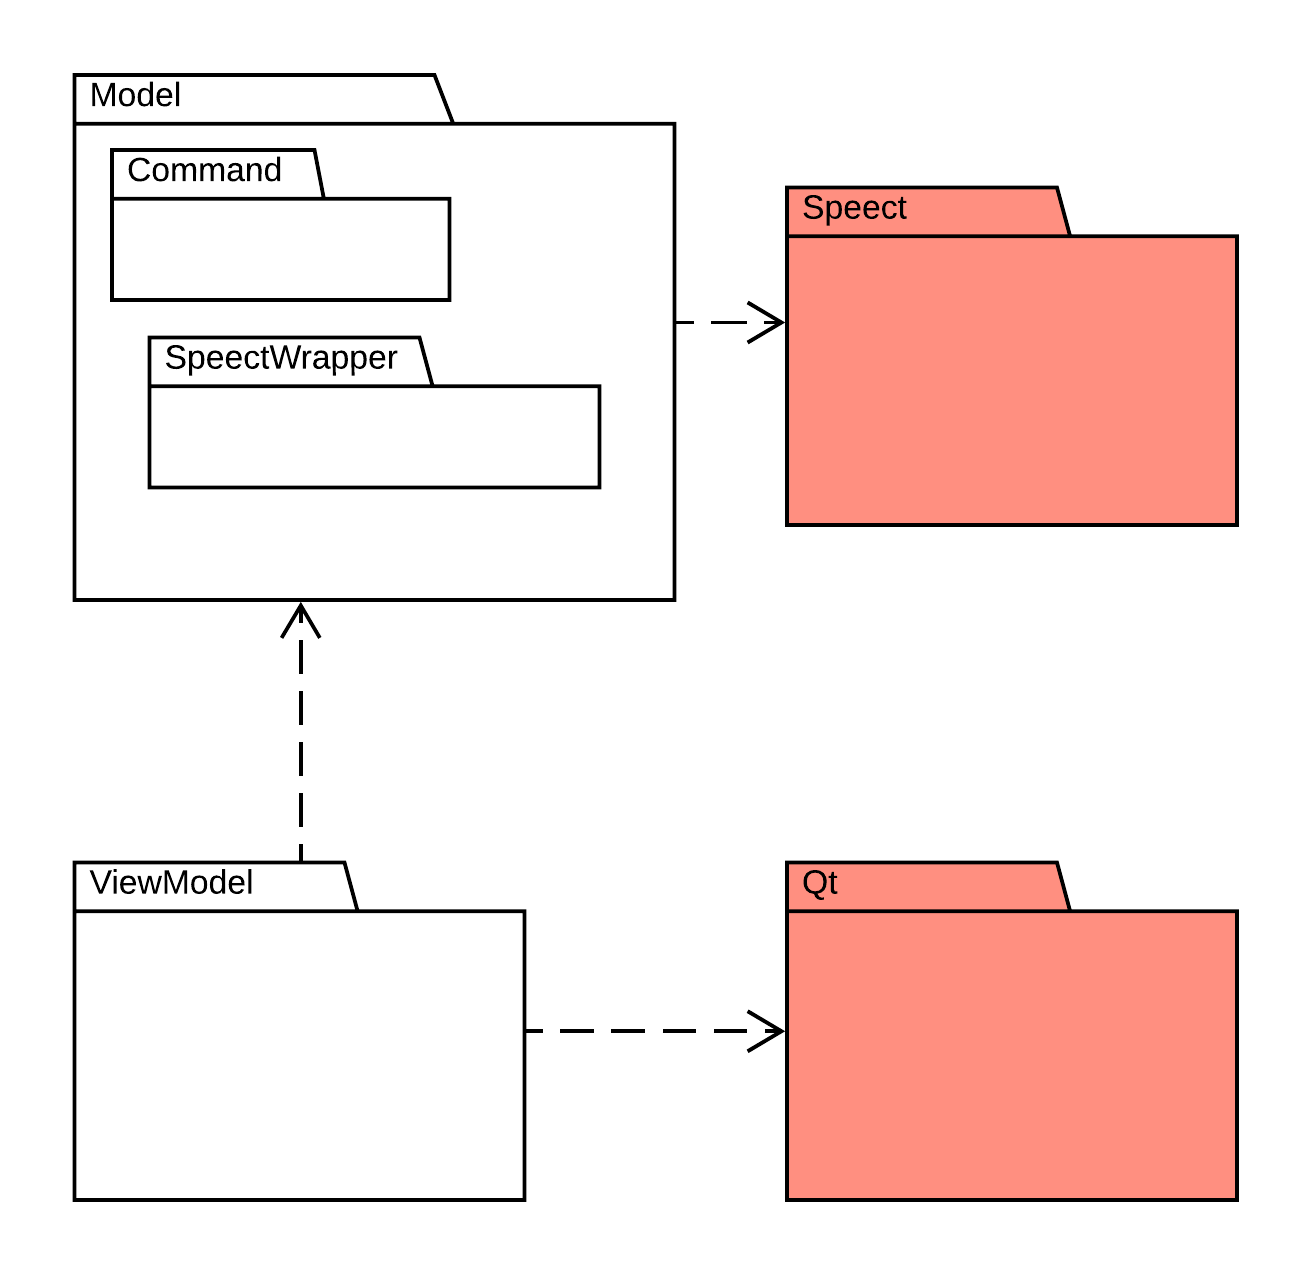
\includegraphics[scale=1.4]{PackageDiagram1}
	\centering
	\caption{Diagramma generale dei package}
\end{figure}

\newpage

\begin{figure}[H]
	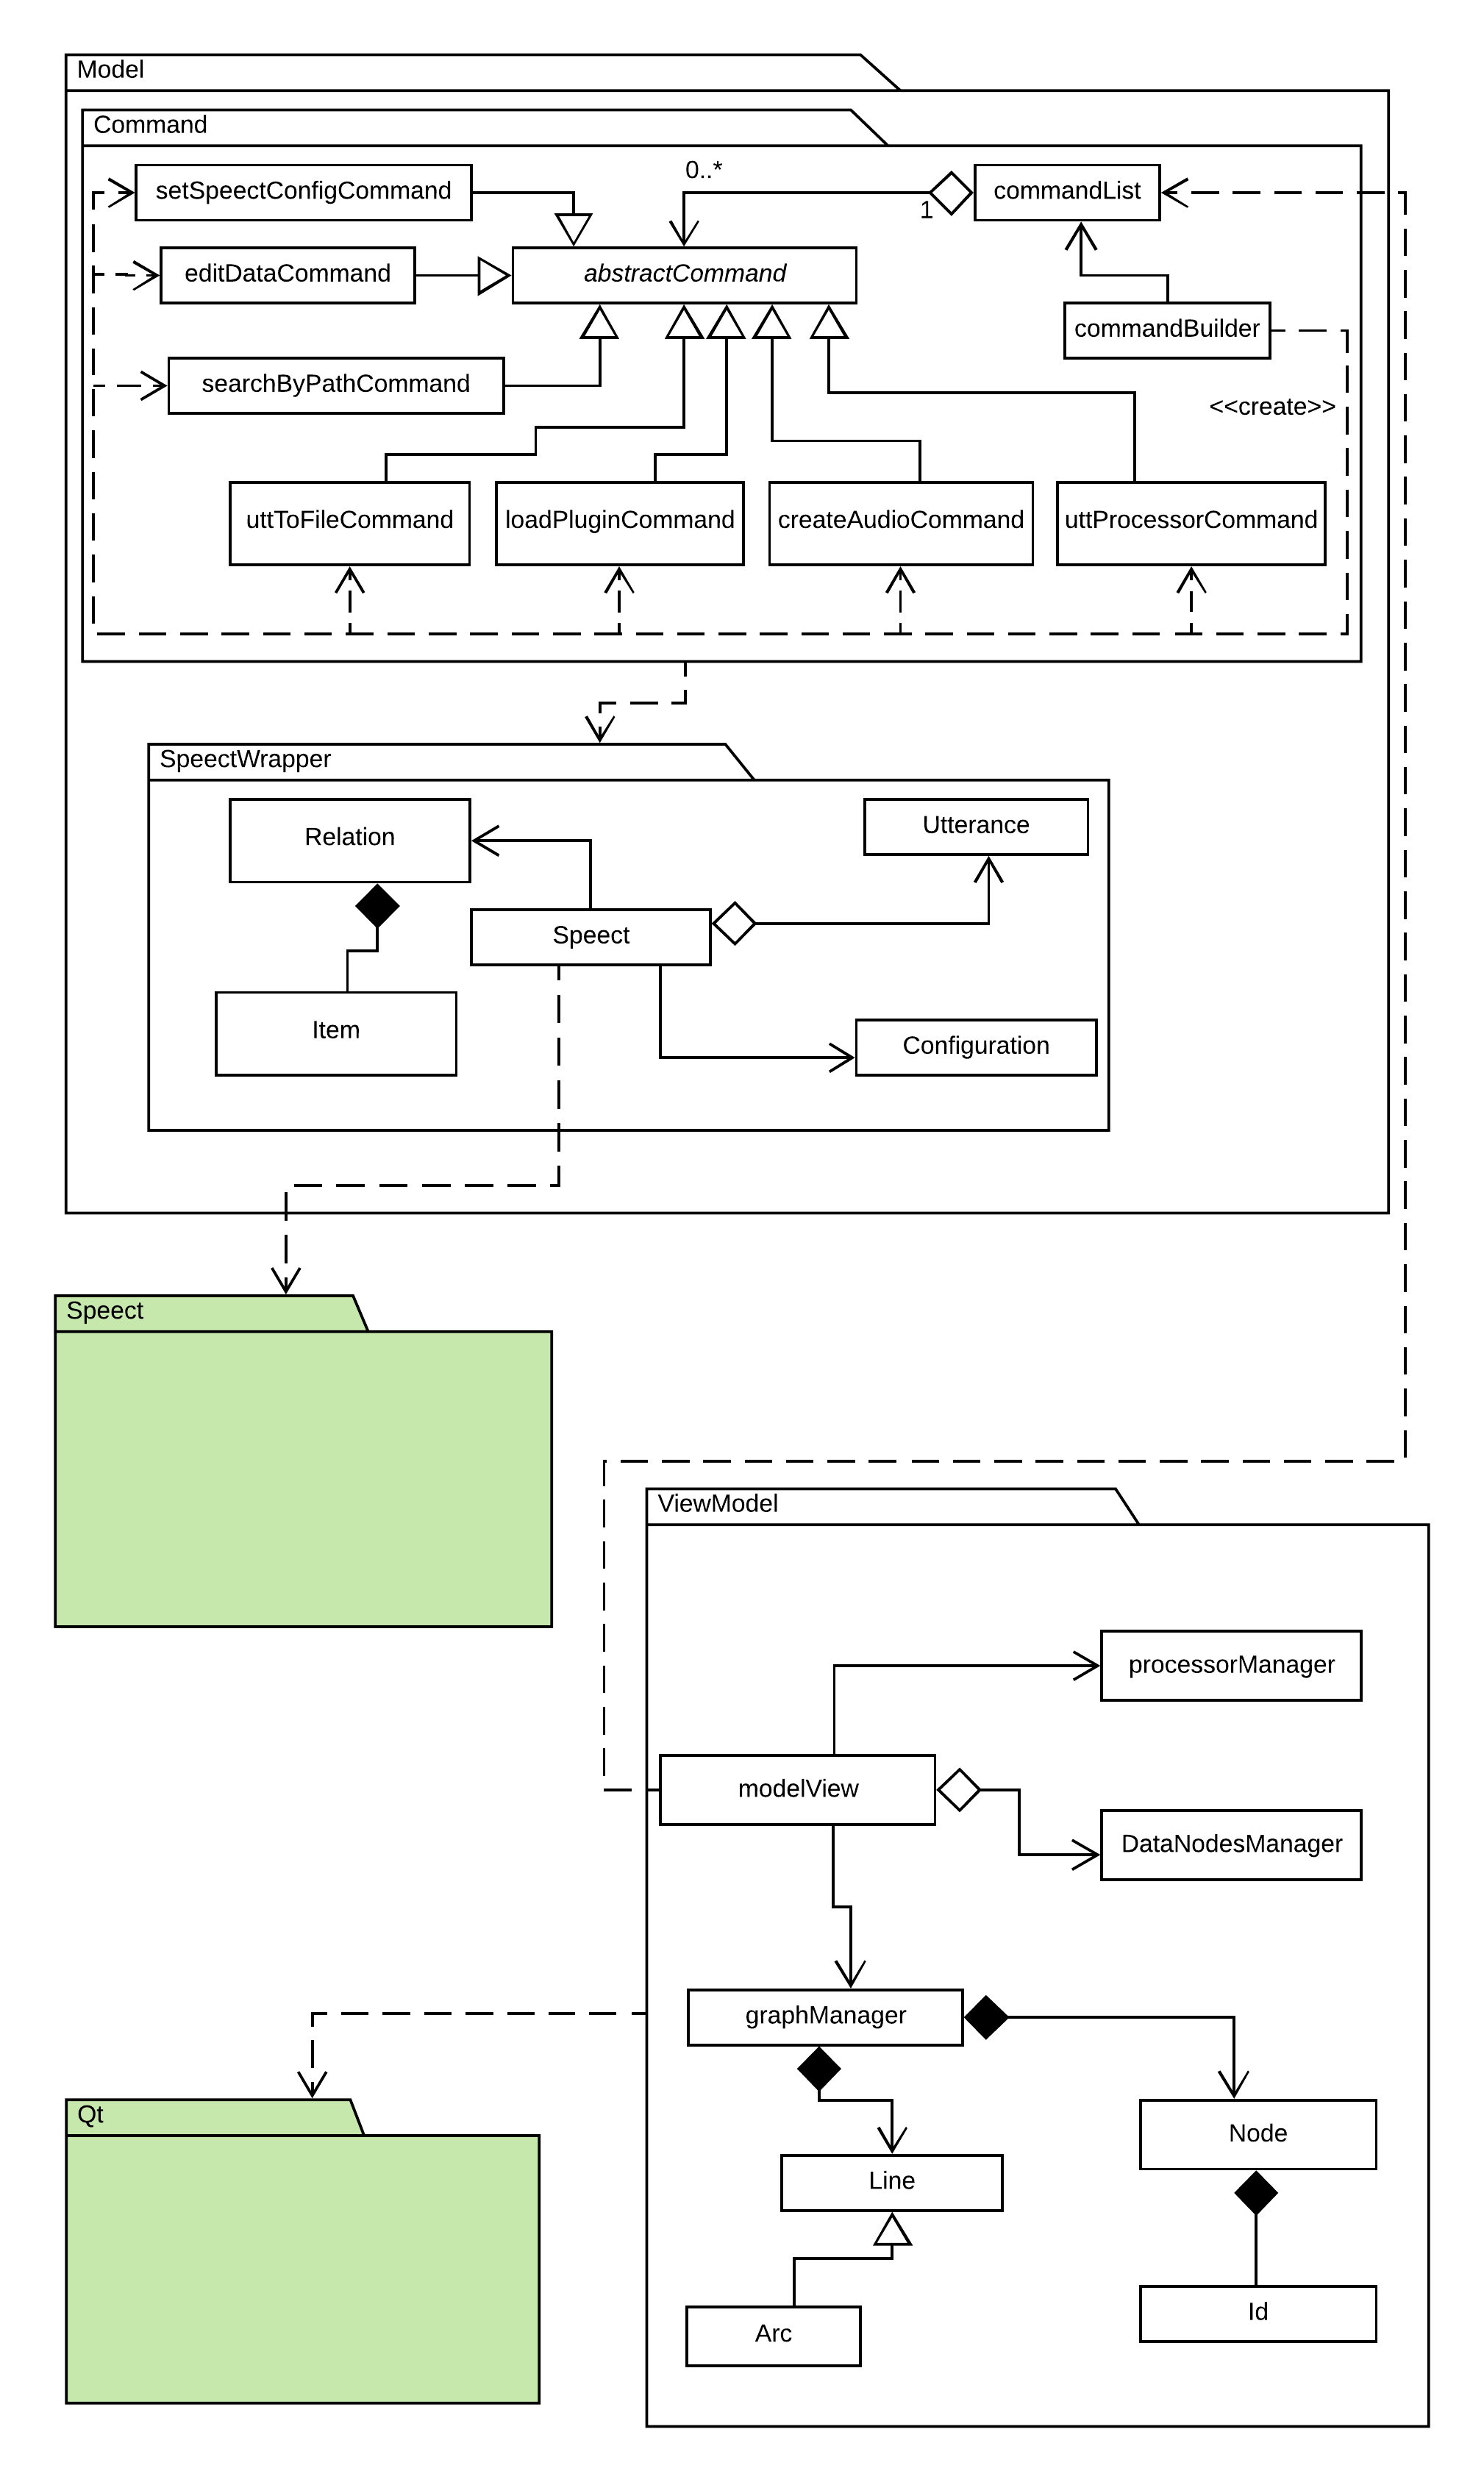
\includegraphics[scale=0.63]{PackageDiagram2}
	\centering
	\caption{Diagramma dei package nel dettaglio}
\end{figure}

\chapter{Implementazione MVVM}

Vengono di seguito illustrate le implementazioni per le componenti del pattern Model-View-ViewModel in relazione all'architettura della Product Baseline. Per ogni componente, vengono illustrati:

\begin{itemize}
	\item \textbf{Contestualizzazione}: spiegazione generale dell'architettura del componente all'interno del sistema.
	\item \textbf{Diagramma delle classi}: diagramma generale delle classi per il componente;
	\item \textbf{Dettaglio delle classi}
	\item \textbf{Design Pattern}: una descrizione e contestualizzazione esaustiva dei design pattern impiegati all'interno del componente.
\end{itemize} 

\section{View}

La View, conseguentemente all’uso del framework Qt, consiste di un file \textit{qml} trasformato durante la compilazione in classi compatibili C++. Il comportamento della View è indi gestito dal package ViewModel. 

\section{Model}

\subsection{Contestualizzazione}

Nella progettazione del Model è emersa la necessità di interagire con la libreria Speect incapsulandone alcune funzionalità rilevanti. Per realizzare ciò il Model è stato diviso in due package corrispondenti all'implementazione dei design pattern Façade (SpeectWrapper), per quanto riguarda l'incapsulamento della libreria, e Command, per quanto riguarda la suddivisione delle funzionalità implementate in un'ottica di componibilità ed estendibilità.  

\subsection{Diagramma delle classi}

\begin{figure}[H]
	\hspace*{-20mm}
	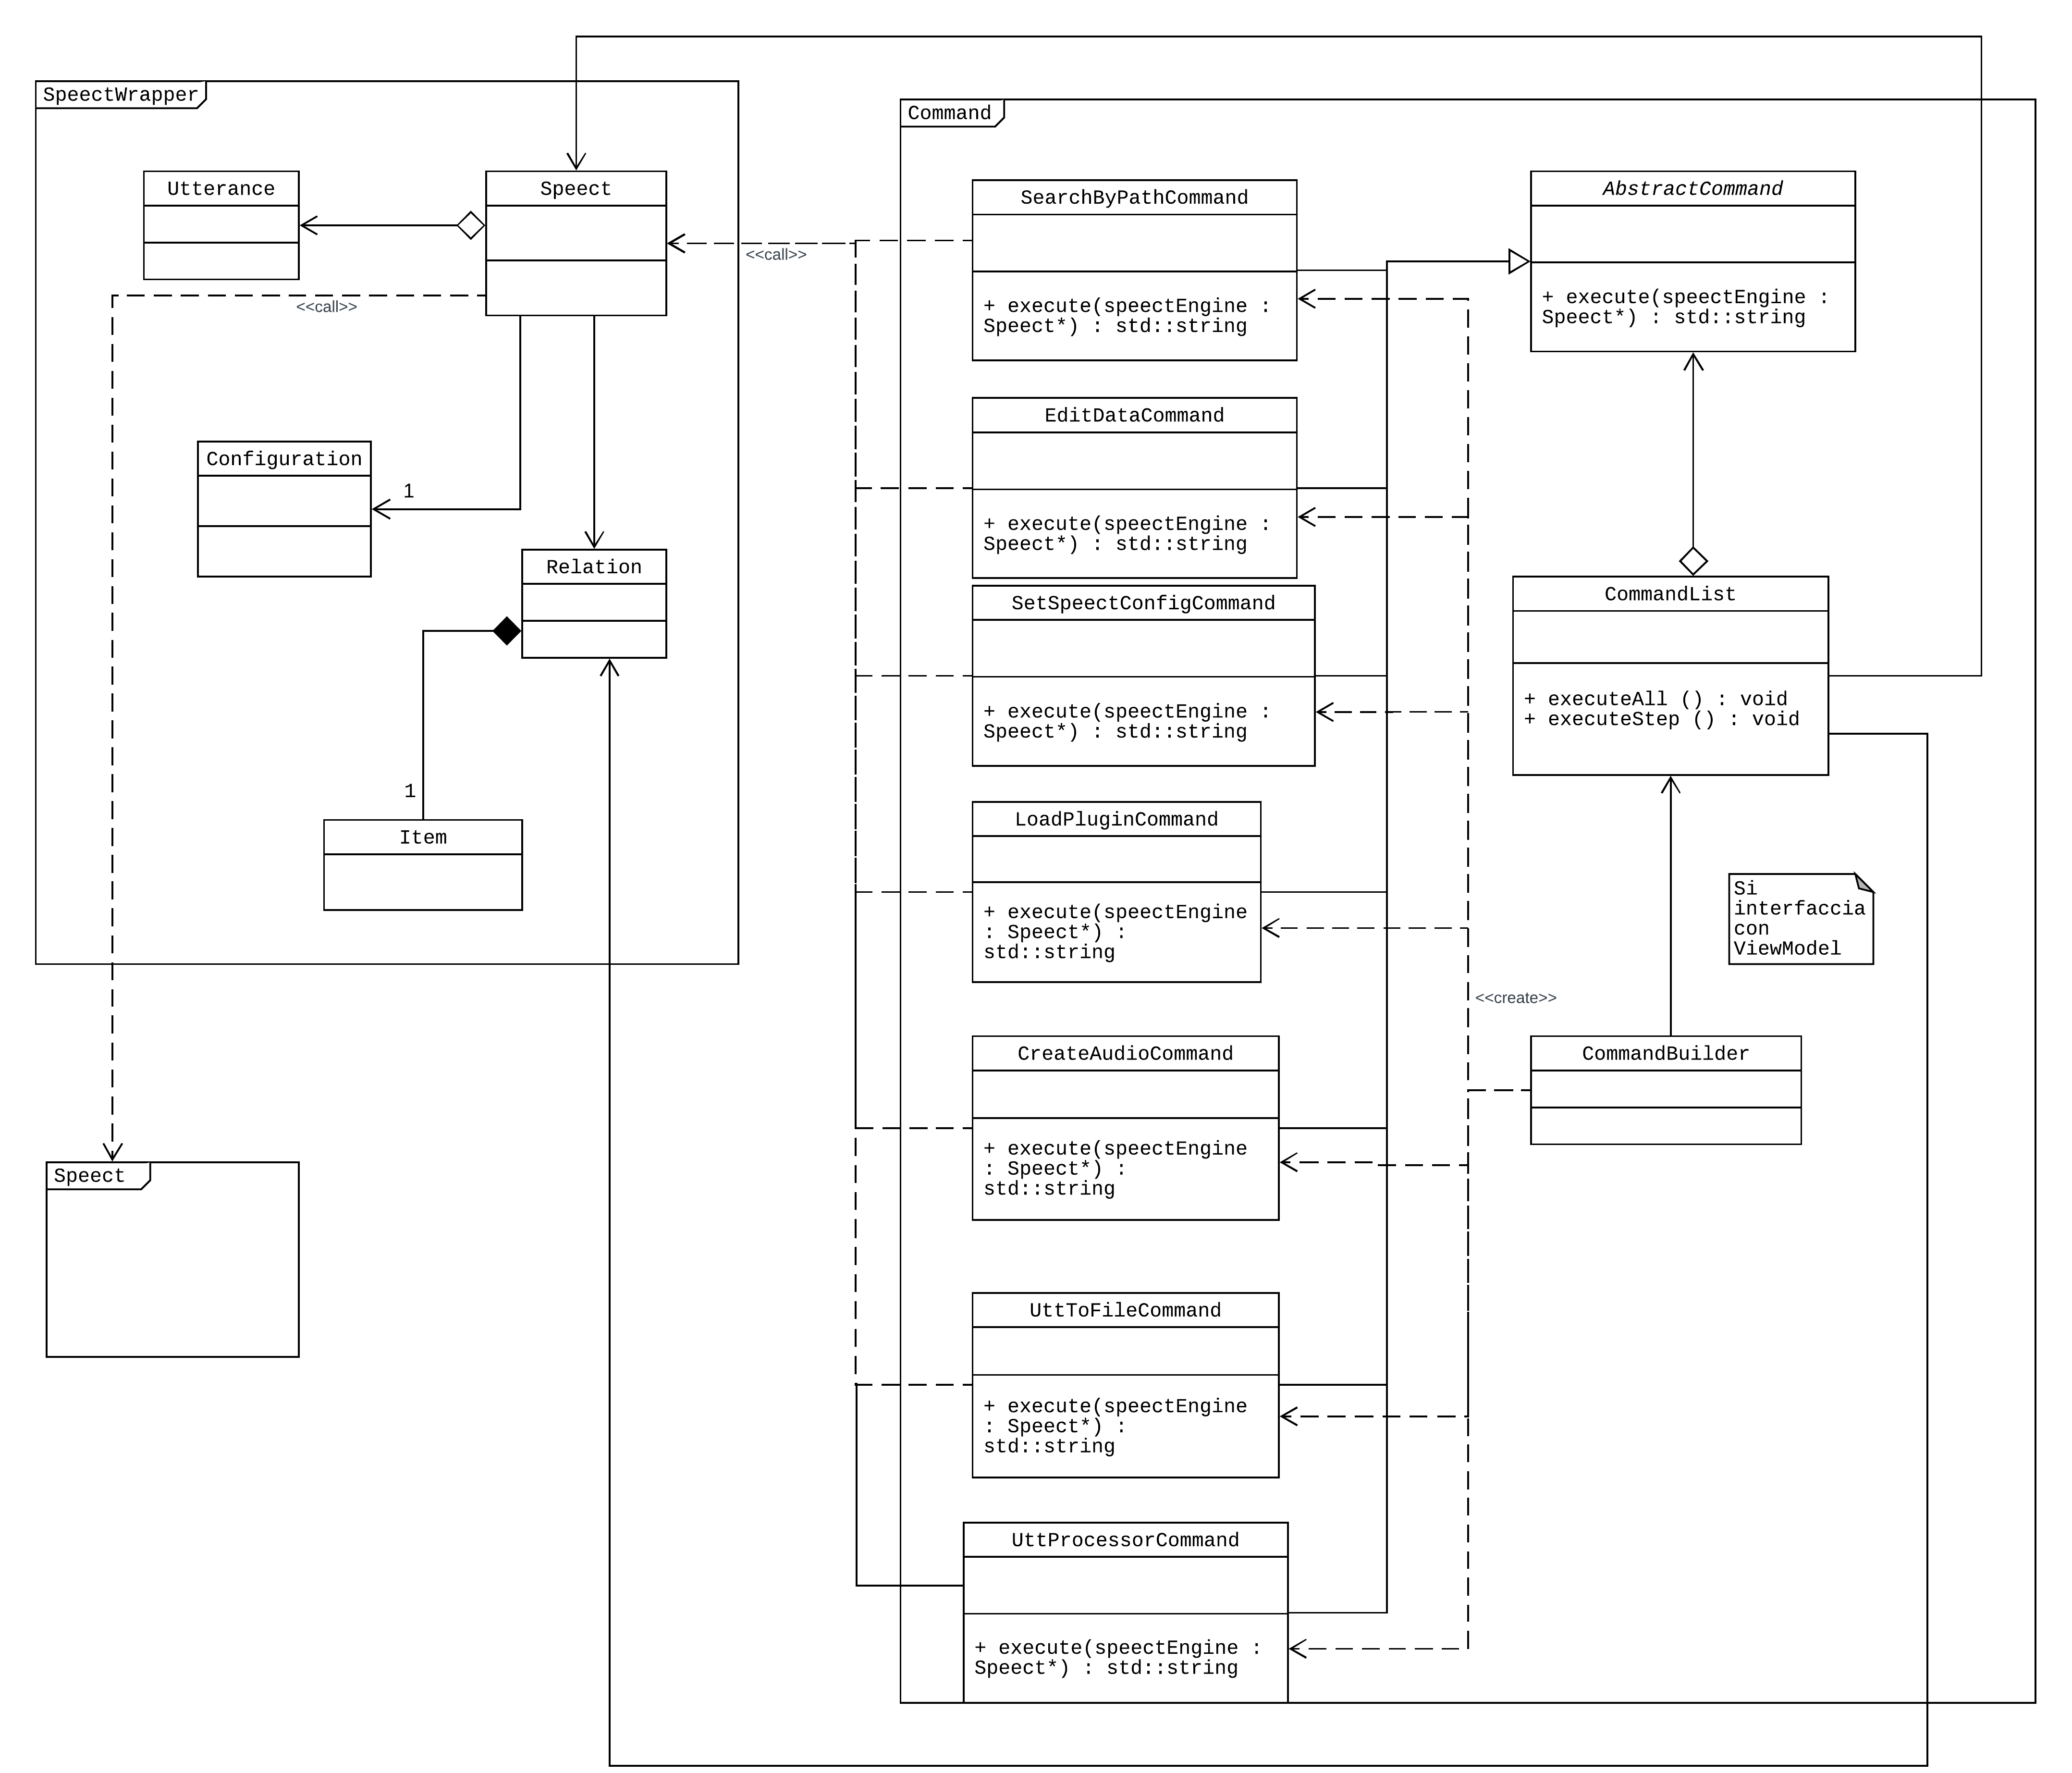
\includegraphics[scale=0.5]{ModelDiagram}
	\centering
	\caption{Diagramma delle classi del componente Model}
\end{figure}

\subsection{Dettaglio delle classi}

Nelle sezioni successive vengono illustrate le classi costituenti il componente Model del prodotto. Tali classi sono aggregate in due principali package:
\begin{itemize}
	\item \textbf{SpeectWrapper}: incapsula la libreria Speect gestendone la memoria. 
	\item \textbf{Command}: offre la possibilità di creare i comandi che, aggregando funzioni Speect, rappresentano le funzionalità base di DeSpeect.
\end{itemize}

\subsubsection{SpeectWrapper}

\begin{itemize}
	\item \textbf{Speect}: incapsula le componenti base della libreria Speect e ne gestisce la memoria;
	\item \textbf{Configuration}: incapsula la configurazione della libreria Speect per garantirne il corretto funzionamento;
	\item \textbf{Utterance}: incapsula i dati relativi all'\glossario{utterance}{utterance} e ne gestisce la memoria;
	\item \textbf{Relation}: incapsula i dati relativi alla \glossario{relation}{relation} e ne gestisce la memoria;
	\item \textbf{Item}: un'iteratore per scorrere una relation di Speect, fornendo inoltre un path relativo al nodo di partenza per raggiungere il nodo attualmente selezionato. 
\end{itemize}

\subsubsection{Command}

\begin{itemize}
	\item \textbf{AbstractCommand}: definisce l'interfaccia base di un comando;
	\item \textbf{CommandList}: aggrega i comandi in una lista, di cui permette l'esecuzione completa o step-by-step;
	\item \textbf{CommandBuilder}: permette la costruzione di una CommandList;
	\item \textbf{SearchByPathCommand}: implementazione del comando che esegue la ricerca di un nodo dato un path;
	\item \textbf{EditDataCommand}: implementazione del comando che esegue la modifica dei dati relativi ad un nodo;
	\item \textbf{SetSpeectConfigCommand}: implementazione del comando che esegue l'impostazione di una data configurazione di Speect;
	\item \textbf{LoadPluginCommand}: implementazione del comando che esegue il caricamento di un plugin;
	\item \textbf{CreateAudioCommand}: implementazione del comando che genera il file audio dall'utterance attuale;
	\item \textbf{UttToFileCommand}: implementazione del comando che esegue il salvataggio dell'utterance in un file secondo il formato desiderato;
	\item \textbf{UttProcessorCommand}: implementazione del comando che esegue un dato utterance processor.
\end{itemize}

\newpage

\subsection{Design pattern}

\subsubsection{Command}
Permette la suddivisione delle funzionalità implementate in un'ottica di componibilità ed estendibilità. I comandi concreti sono aggregati in una lista (\verb|CommandList|) che si interfaccia con la componente ViewModel. Tali comandi interagiscono a loro volta con il package SpeectWrapper per ottere i dati da elaborare dalla libreria Speect. Ai comandi è delegata l'esecuzione degli utterance processor per la successiva stampa dei dati nel grafo, ma anche l'implementazione di funzionalità quali il caricamento dei \glossario{plug-in}{plug-in} e della configurazione di Speect.

\subsubsection{Builder}
Questo design pattern separa la costruzione di un oggetto complesso dalla sua rappresentazione, cosicché il processo di costruzione stesso possa creare diverse rappresentazioni. Contestualizzato nel sistema della PB, esso si interfaccia con il ViewModel per la configurazione e costruzione di una specifica \verb|CommandList|.

\subsubsection{Façade} 
Il design pattern Façade permette, attraverso un'interfaccia più semplice, l'accesso a sottosistemi che espongono interfacce complesse e molto diverse tra loro, nonché a blocchi di codice complessi. In questo contesto, il package SpeectWrapper incapsula la libreria Speect rendendola accessibile tramite omonima classe proprietaria.

\newpage

\section{ViewModel}

\subsection{Contestualizzazione}
Il package ViewModel funge da tramite tra Model e View, prelevando i dati dal primo per aggiornare il secondo. Per quanto riguarda la stampa del grafo, la classe \verb|GraphManager| si occupa di aggiornarne la presentazione interfacciandosi con le librerie Qt e con le classi \verb|Line|, \verb|Arc| e \verb|Node|.  

\subsection{Diagramma delle classi}

\begin{figure}[H]
	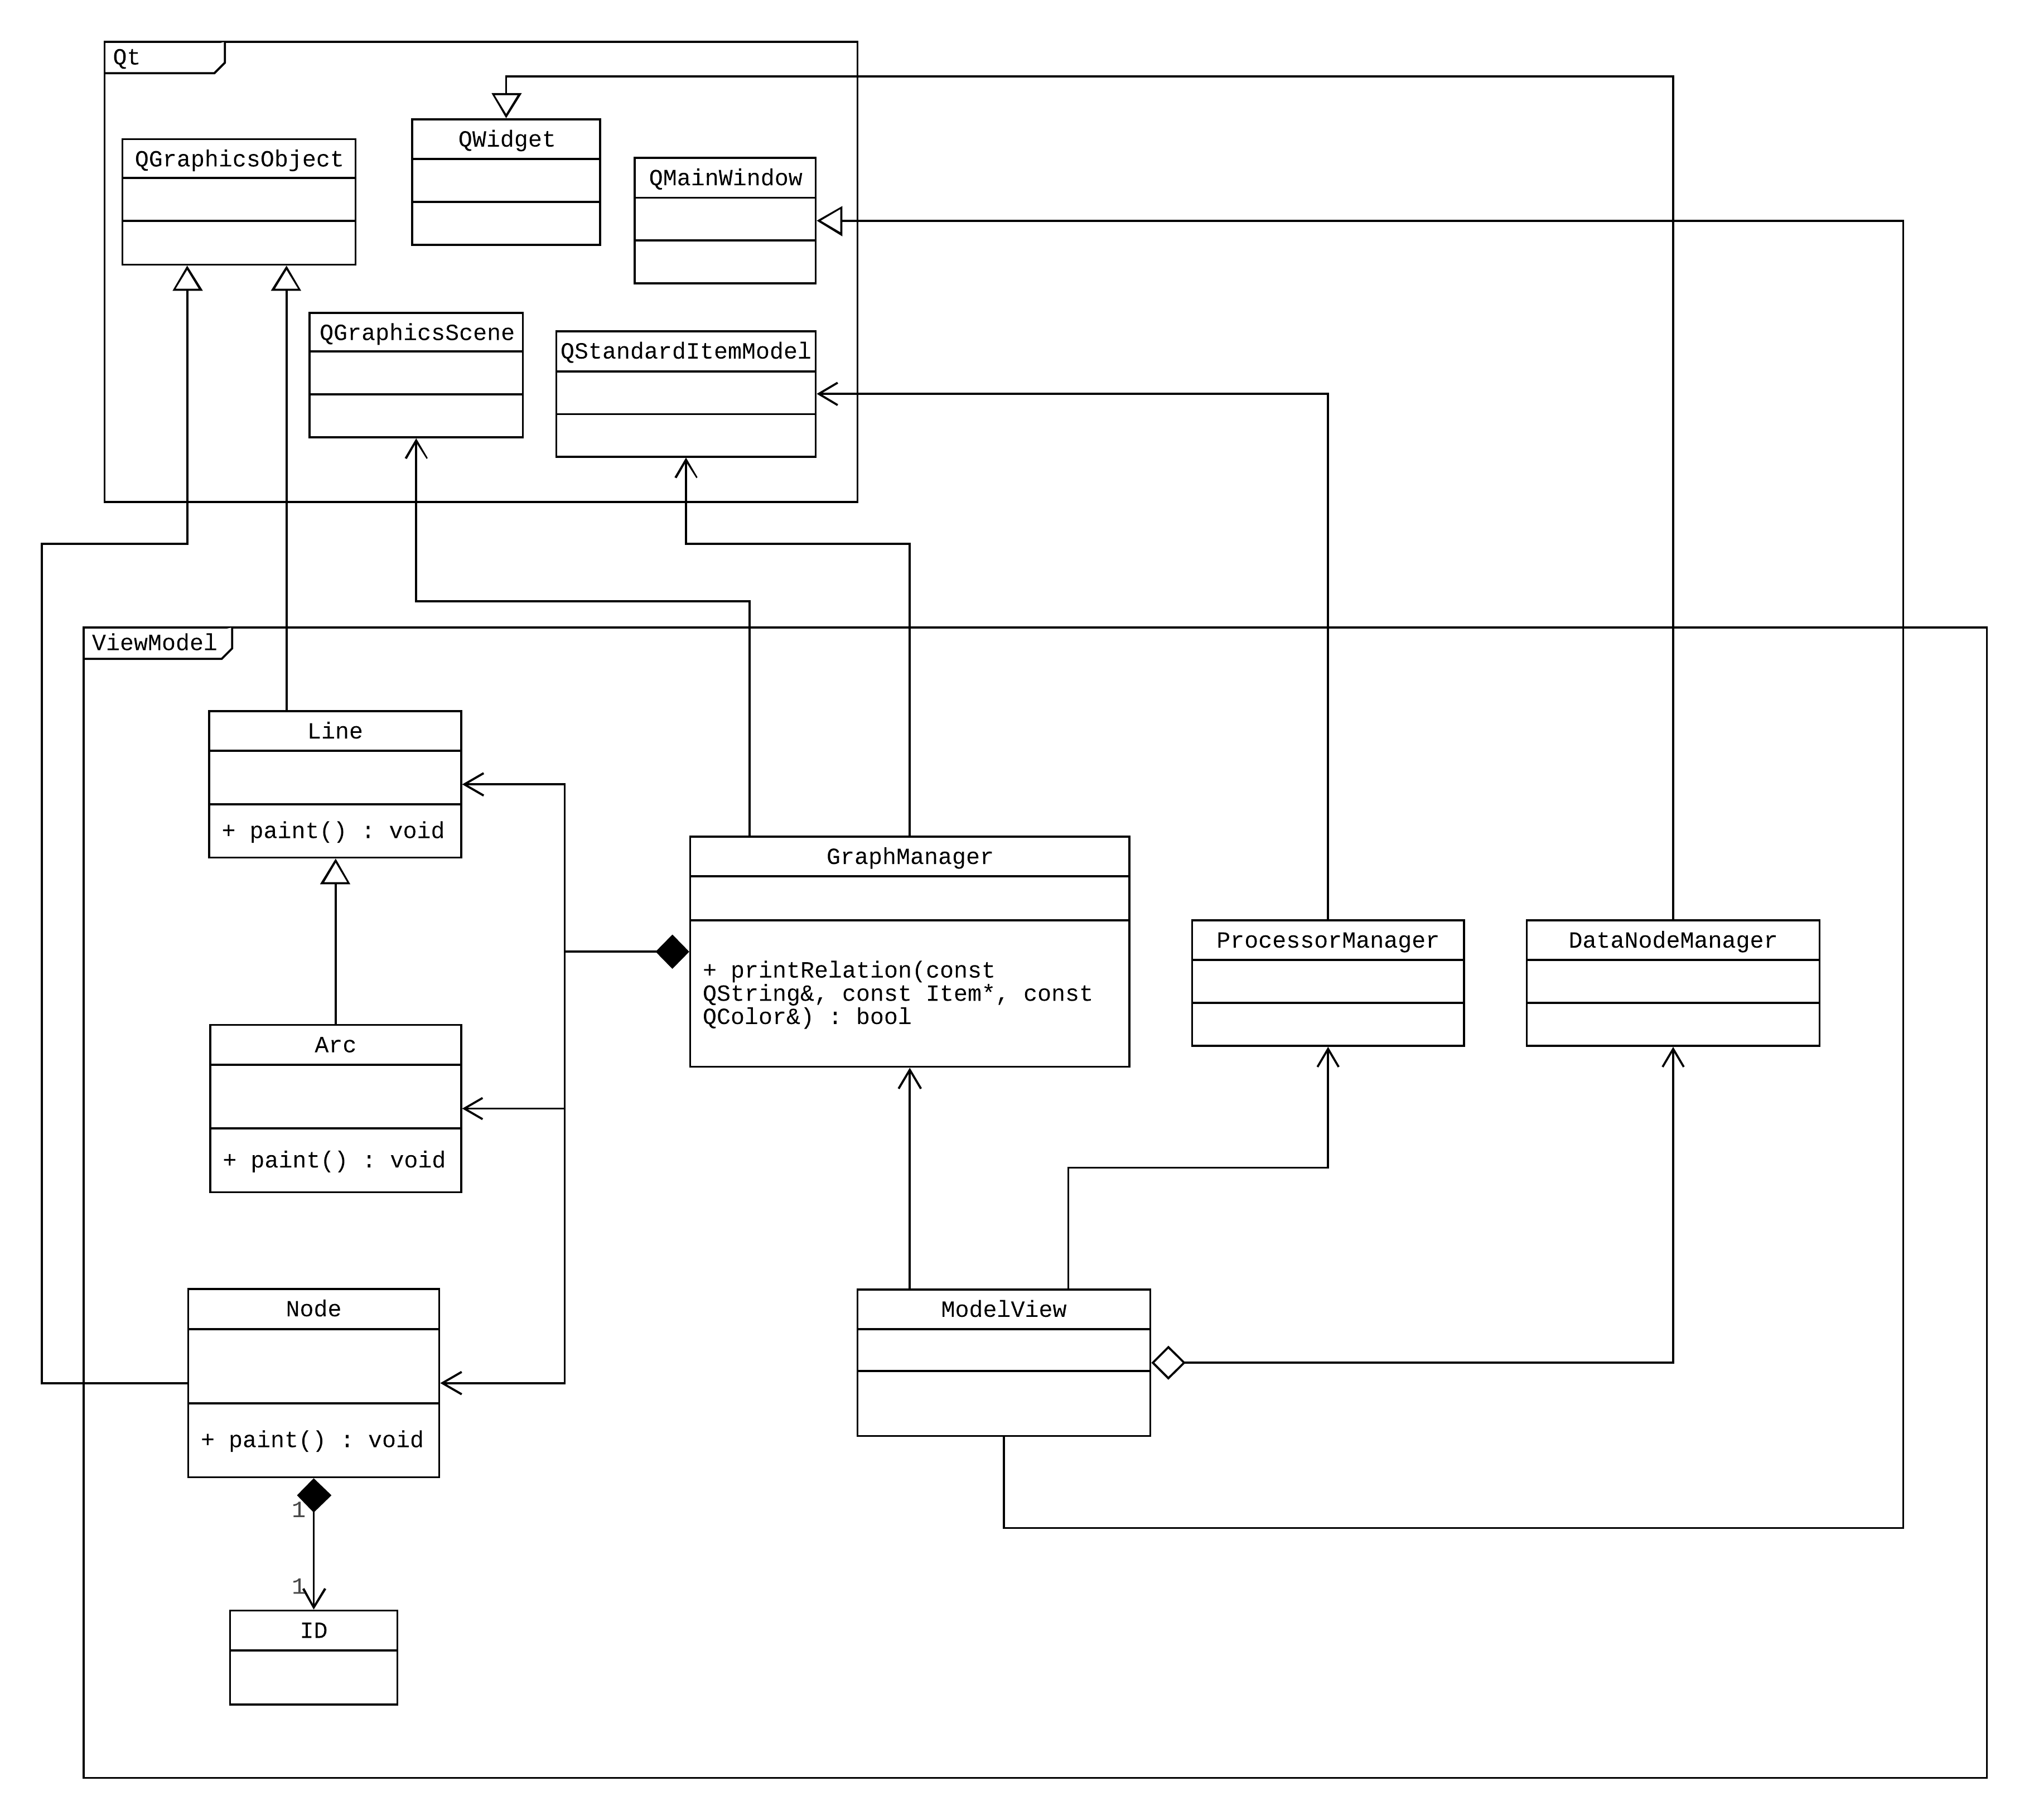
\includegraphics[scale=0.5]{ViewModelDiagram}
	\centering
	\caption{Diagramma delle classi del componente ViewModel}
\end{figure}

\subsection{Dettaglio delle classi}

Nelle sezione successive verranno illustrate le classi che costituiscono il package ViewModel.

\subsubsection{ViewModel}

\begin{itemize}
	\item \textbf{ModelView}: gestisce le richieste fatte dal client tramite la View;
	\item \textbf{GraphManager}: gestisce il modello del grafo;
	\item \textbf{ProcessorManager}: gestisce la selezione dei processor per l'esecuzione;
	\item \textbf{DataNodeManager}: gestisce i dati relativi ad uno specifico nodo;
	\item \textbf{Line}: modella una linea;
	\item \textbf{Arc}: modella un arco orientato del grafo;
	\item \textbf{Node}: modella un nodo del grafo;
	\item \textbf{ID}:  rappresenta una struttura dati che definisce l'identificatore specifico di un nodo.
\end{itemize}

\subsection{Design pattern}

\subsubsection{Observer}
Il framework Qt, attraverso il sistema di signal e slot, implementa tale design pattern. Esso permette di reagire efficientemente ad un cambiamento dell'interfaccia grafica, chiedendo se necessario l'aggiornamento dei dati del Model attraverso il ViewModel. Il meccanismo di signal e slot è implementato dalle classi pertinenti all'interno del package.  

\newpage
		
	\chapter{Estensione delle funzionalità}
	
	\section{Modificare l'interfaccia grafica}
	Per modificare l'attuale interfaccia grafica, è sufficiente apportare le modifiche desiderate al file qml \verb|view.ui| contenuto in \verb|DeSpeect/Qt/src/|. Le modifiche da apportare a tale file vanno eseguite tramite Qt Creator, ulteriori informazioni riguardo i file qml sono reperibili al seguente link:
	\begin{center}
		\url{https://doc.qt.io/qt-5.10/qtqml-index.html}
	\end{center}

	\noindent Qualora le modifiche all'interfaccia grafica corrispondano all'implementazione di nuove funzionalità, è necessario estendere i package Model e ViewModel per garantirne la coerenza.
	
	\section{Aggiungere un plug-in}
	L'architettura di DeSpeect prevede un apposito comando per il caricamento di nuovi plug-in all'interno del package Command. Qualora il plug-in richiedesse l'invocazione di metodi specifici, sarà necessario incapsularli in un nuovo comando che definisce la corretta procedura d'esecuzione del plug-in stesso. Sarà dunque necessario implementare un nuovo comando concreto estendendo la classe AbstractCommand. Maggiori informazioni su struttura e funzionamento dei plug-in di Speect sono reperibili all'interno della documentazione ufficiale, nello specifico al seguente link:
	\begin{center}
		\url{http://speect.sourceforge.net/topics/plugins_topic.html}
	\end{center}
	
	\chapter{Verifica delle estensioni}
	
	\section{Aggiungere un test}
	
	Quando DeSpeect viene esteso con una nuova funzionalità è opportuno creare i relativi test di unità per verificarne la correttezza. I test per DeSpeect sono implementati mediante la tecnologia Google Test, come citato in §3.2.1 di questo documento. Per completezza viene di seguito riportato il link alla documentazione di tale tecnologia:
	\begin{center}
		\url{https://github.com/google/googletest/blob/master/googletest/docs/Primer.md}
	\end{center}
	Si rimanda a tale documentazione per la corretta sintassi e configurazione dei file di test, che vanno inseriti nella cartella \verb|DeSpeect/Test/| del progetto affinché vengano correttamente eseguiti automaticamente da Travis CI (tecnologia approfondita in §3.2.2 di questo documento). 
	
	\section{Eseguire un test}
	
	\subsection{Esecuzione automatica dei test}
	Il servizio Travis CI, integrato con il repository GitHub relativo al progetto, testa la build ed esegue i test automaticamente ad ogni modifica del codice sul repository. Lo stesso rilascia successivamente i dati sul \textit{code coverage} al servizio web \textit{coveralls.io}, anch'esso collegato al repository GitHub, che aggiorna così i propri report. É possibile prendere spunto dal file \verb|.travis.yml| presente nel repository e dalla documentazione reperibile al link:
	\begin{center}
		\url{https://docs.travis-ci.com/user/languages/cpp/}
	\end{center}
	Per predisporre il proprio sistema di integrazione continua con Travis CI qualora non si volesse creare una fork del progetto originale. Per la corretta integrazione del testing con Google Test e coveralls.io si suggerisce la presa visione della seguente documentazione esemplificativa:
	\begin{center}
		\url{https://github.com/bast/gtest-demo}
	\end{center} 
	
	\subsection{Esecuzione manuale dei test}
	A seguito dell'esecuzione dello script \verb|build.sh| citato in §4.1 di questo documento viene generata automaticamente una build e un'esecuzione dei test contenuti nella directory \verb|DeSpeect/Test/|. I test sono eseguibili sia con il comando \verb|ctest| che con il comando \verb|unit_tests| e la loro esecuzione mostra sinteticamente il code coverage relativo. 
	
	\appendix
	
	\chapter{Model-View-ViewModel}
	
	\section{Struttura del pattern}
	
	Il design pattern architetturale \textit{Model-View-ViewModel} (MVVM in breve) facilita la separazione dell'interfaccia grafica, che si tratti di linguaggio di markup o codice GUI, dallo sviluppo della logica di business o della logica di back-end, ovvero dal modello dei dati. Il \textit{view model} di MVVM è un convertitore di valori, nel senso che il view model è responsabile dell'esposizione (conversione) degli oggetti dati dal modello così da renderli facilmente gestibili e presentabili. In quest'ottica, la view è più un modello che una vista e gestisce la maggior parte se non tutta la logica di visualizzazione della vista. Il pattern è riassunto dal seguente schema ed i suoi componenti principali sono di seguito approfonditi.
	
	\begin{figure}[H]
		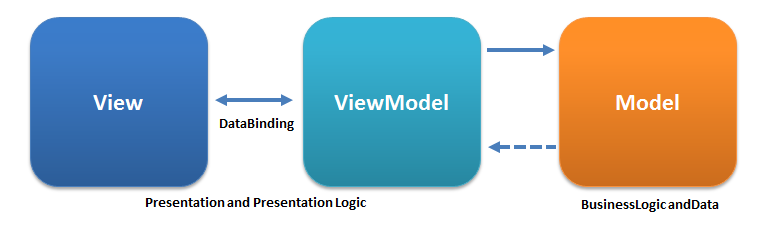
\includegraphics[scale=0.7]{MVVMPattern}
		\centering
		\caption{Diagramma generale dell'architettura MVVM}
	\end{figure}
	
	\noindent I tre componenti principali dell'architettura sono i seguenti:
	\begin{itemize}
		\item \textbf{Model}: il \textit{Model} (o modello) è un'implementazione del modello di dominio dell'applicazione ed include un modello dei dati affiancato alla logica di business e di validazione;
		\item \textbf{View}: la \textit{View} (o vista) è responsabile della definizione della struttura, del layout e dell'aspetto di ciò che l'utente visualizza su schermo. Idealmente, la vista è definita puramente con linguaggio di markup o generico codice GUI che non contiene la logica di business;
		\item \textbf{ViewModel}: la \textit{ViewModel} (o modello di presentazione) funge da intermediario tra la vista e il modello ed è responsabile della gestione della logica di visualizzazione. In genere, il ViewModel interagisce con il modello richiamandone i metodi delle classi: esso fornisce quindi dati dal modello in una forma facilmente utilizzabile dalla View. Il ViewModel recupera i dati dal modello, rendendoli disponibili alla View, e può riformattarli in un modo che renda più semplice la gestione della vista. Esso fornisce anche l'implementazione dei comandi che un utente dell'applicazione avvia nella vista (ad esempio, quando un utente clicca un pulsante nell'interfaccia grafica, tale azione può attivare un comando nel ViewModel) e può essere responsabile della definizione delle modifiche dello stato logico che influiscono su alcuni aspetti della visualizzazione nella vista, ad esempio l'indicazione che alcune operazioni sono in sospeso.
	\end{itemize}
	
	\section{Vantaggi offerti dal pattern}
	Il MVVM offre i seguenti vantaggi:
	
	\begin{itemize}
		\item Durante il processo di sviluppo, i programmatori e i designer possono lavorare in modo indipendente e simultaneamente sui loro componenti. Quest'ultimi possono concentrarsi sulla vista e, utilizzando appositi strumenti, generare facilmente dati di esempio con cui lavorare, mentre i programmatori possono lavorare sul modello di presentazione e sui componenti del modello;
		\item Gli sviluppatori possono creare test unitari per il ViewModel e per il Model senza utilizzare la View;
		\item È facile riprogettare l'interfaccia grafica dell'applicazione senza toccare il resto del codice, una nuova versione della vista dovrebbe poter funzionare con il modello di presentazione esistente;
		\item Se esiste un'implementazione del modello che incapsula la logica di business, potrebbe essere difficile o rischioso cambiarla. In questo scenario, il ViewModel funge da adattatore per le classi del Model e consente di evitare modifiche importanti al codice dello stesso.	
	\end{itemize}

	\chapter{Contribuire a DeSpeect}
	
	DeSpeect è software open source e permette quindi di
	essere modificato. Se si vuole contribuire al progetto originale è possibile farlo mediante la creazione di fork sul repository GitHub. Risulta inoltre possibile aprire dei ticket per segnalare errori, malfunzionamenti o la richiesta di nuove funzionalità. Il link al repository è il seguente:
	\begin{center}
		\url{https://github.com/graphiteSWE/DeSpeect}
	\end{center}
	
	\begin{figure}[H]
		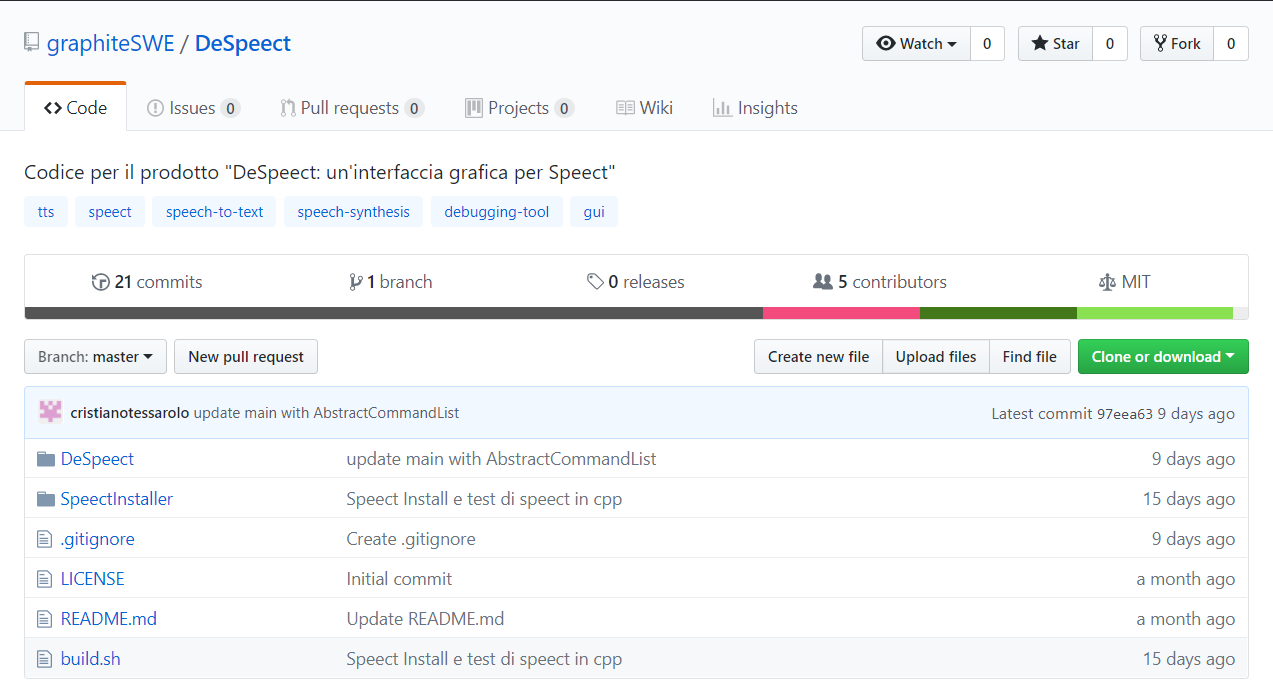
\includegraphics[scale=0.5]{github-home}
		\centering
		\caption{Schermata principale del repository GitHub}
	\end{figure}

	\section{Aprire un ticket}
	
	Per aprire un \textit{ticket} è sufficiente recarsi nella sezione \textit{Issues} del repository GitHub del progetto e cliccare il pulsante \textit{New Issue}. A questo punto verrà chiesto di inserire un titolo e una descrizione per il ticket.
	
	\begin{figure}[H]
		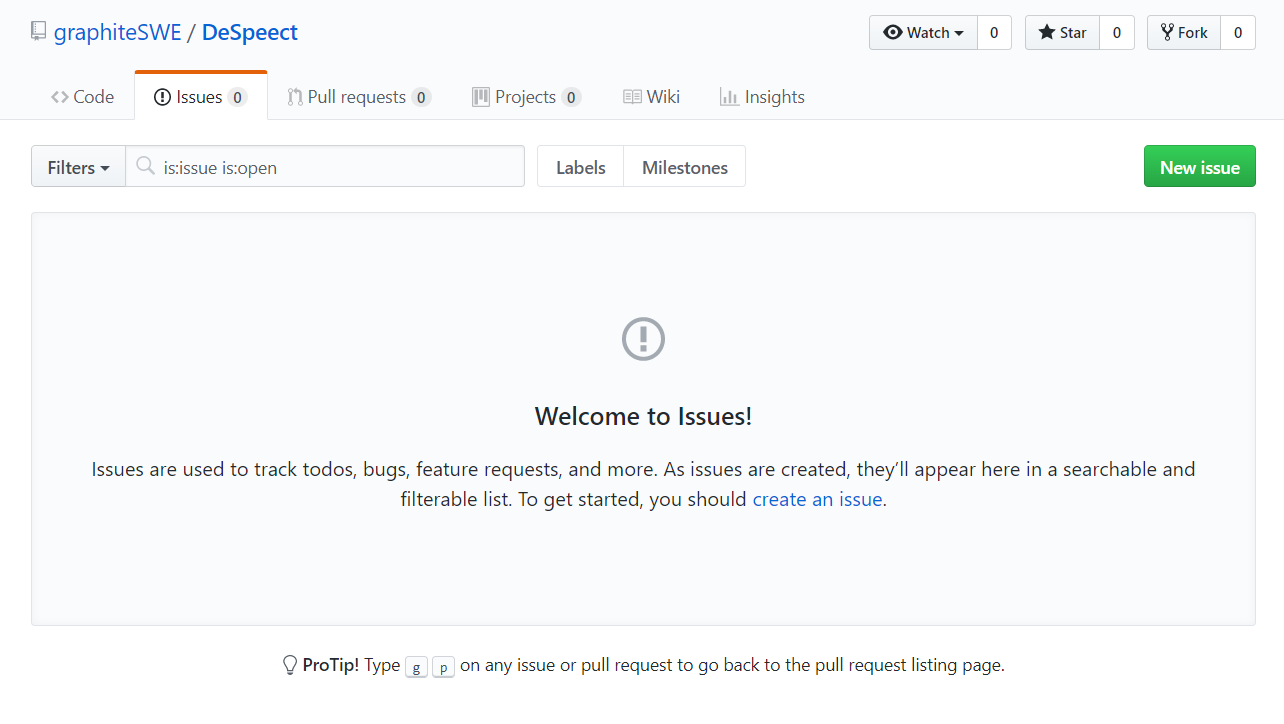
\includegraphics[scale=0.5]{github-new-issue}
		\centering
		\caption{Tab del repository relativa agli issue}
	\end{figure}

	\begin{figure}[H]
		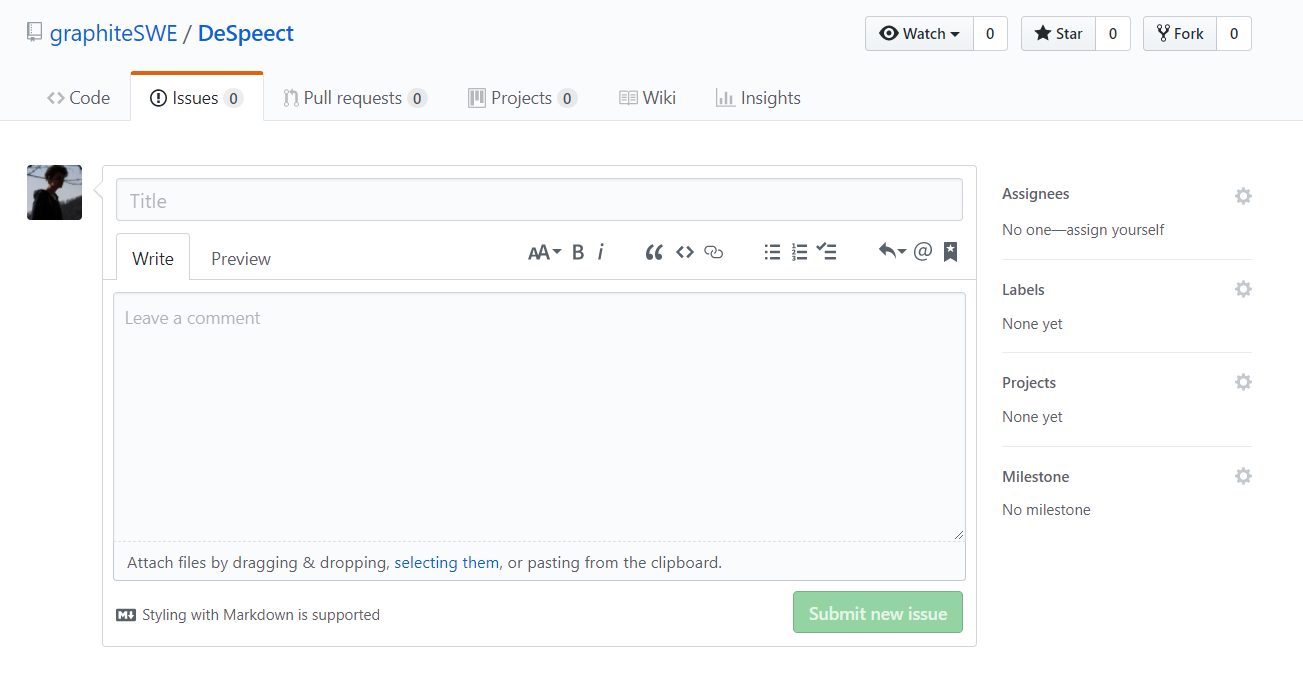
\includegraphics[scale=0.5]{github-new-issue-writing}
		\centering
		\caption{Schermata di scrittura del nuovo issue}
	\end{figure}
	
	Si segnala che è obbligatorio aggiungere allo stesso delle \textit{labels}, atte a rendere facilmente reperibili e categorizzabili i ticket aperti. Un ticket privo di labels
	viene automaticamente rifiutato. 
	Per agevolare la pronta risoluzione di un ticket, si invita a seguire i seguenti accorgimenti:
	\begin{itemize}
		\item Per segnalare un malfunzionamento, comunicare nella descrizione del ticket le seguenti informazioni:
			\begin{itemize}
				\item Sistema operativo completo di specifiche tecniche;
				\item Versione utilizzata di Qt;
				\item Versione utilizzata di CMake;
				\item Versione utilizzata di GCC.
			\end{itemize}
		\item Per richiedere una nuova funzionalità è necessario attendere l'approvazione di uno degli amministratori del repository e l'assegnamento del relativo ticket;
		\item La descrizione del ticket deve essere esaustiva, chiara e rilevante.
	\end{itemize}
	Non rispettare uno dei punti precedenti comporta l'automatica cancellazione del ticket. 
	
	\section{Creare una Pull Request}
	
	Per configurare il progetto DeSpeect è possibile creare una fork del repository originale, il che consente di lavorare in completa autonomia su una certa funzionalità che si vuole aggiungere all'applicazione. In seguito, se si vuole inserire tale funzionalità nel progetto originale, è necessario creare una \textit{Pull Request} all'interno di GitHub. Una volta creata la Pull Request cliccando sulla relativa tab all'interno del repository e successivamente sul pulsante \textit{Create pull request}, è sufficiente attendere l'approvazione di uno degli amministratori del repository originale per poter eseguire il merge delle modifiche.
	
	\begin{figure}[H]
		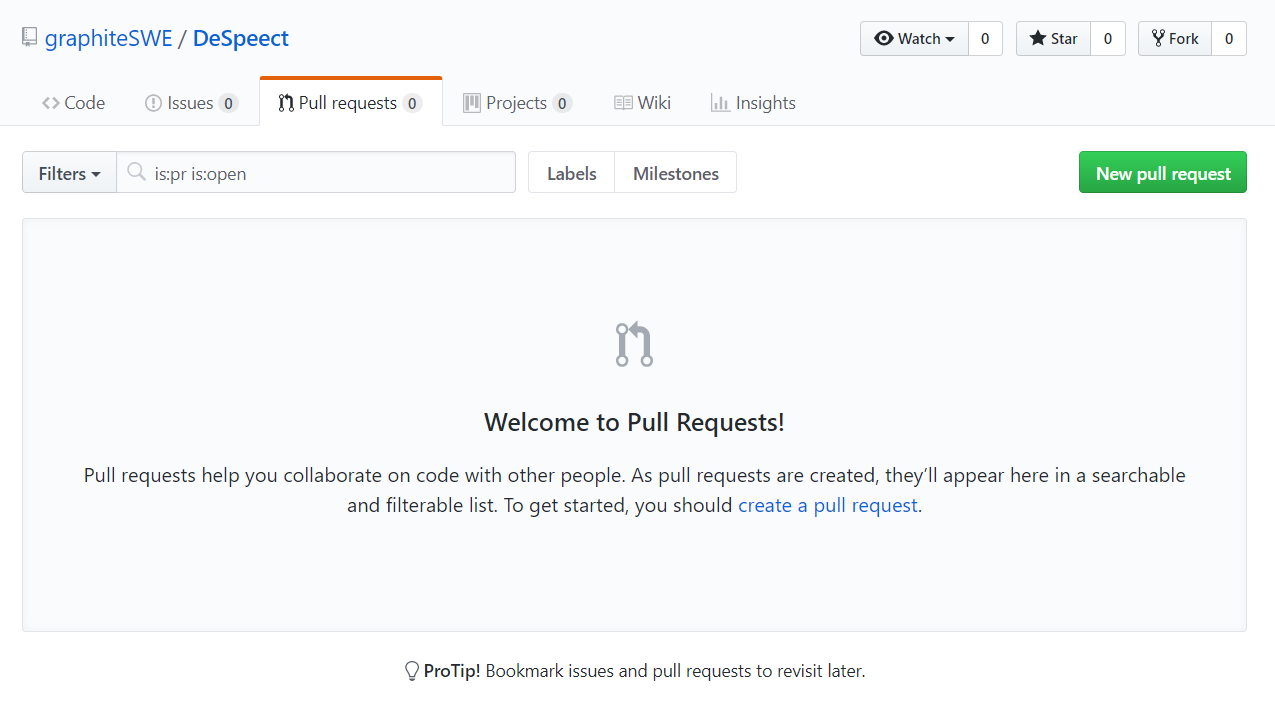
\includegraphics[scale=0.5]{github-new-pull-request}
		\centering
		\caption{Tab del repository relativo alle pull request}
	\end{figure}
	
	\begin{figure}[H]
		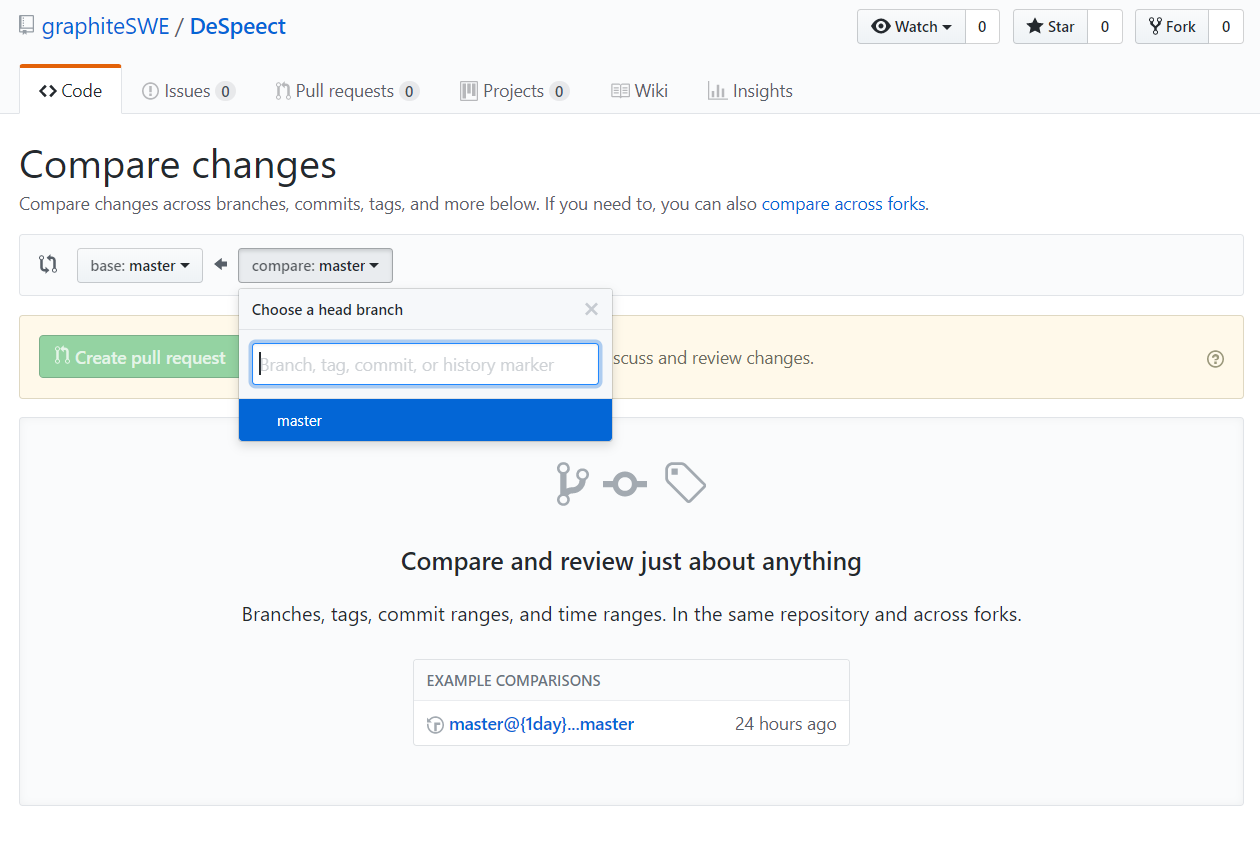
\includegraphics[scale=0.5]{github-new-pull-request-branch}
		\centering
		\caption{Schermata di creazione della pull request e selezione branch}
	\end{figure}

	Di seguito sono riportati i passi da eseguire per creare una Pull
	Request utilizzando la fork di DeSpeect:
	\begin{enumerate}
		\item Creare la fork di DeSpeect;
		\item Recarsi nella sezione \textit{Pull Request} del repository originale;
		\item Selezionare \textit{compare across forks};
		\item Su \textit{base fork} e relativo \textit{base} lasciare invariati i valori inseriti (riguardano il branch master del progetto originale);
		\item Su \textit{head fork} selezionare la propria fork e di conseguenza sul relativo \textit{head} scegliere
		il branch dove sono state apportate le modifiche;
		\item Infine selezionare \textit{Create pull request} aggiungendovi titolo e commento.
	\end{enumerate}
	Anche in questo caso valgono gli stessi accorgimenti illustrati in relazione ai ticket, sintetizzati in descrizioni esaustive, chiare e rilevanti.
	
	\chapter{Licenza}
	
	Il codice di DeSpeect, fatta eccezione per le librerie esterne impiegate (quali Speect e Qt), è rilasciato sotto licenza \textit{MIT}. L'immagine seguente riassume brevemente i punti salienti di tale licenza:
	
	\begin{figure}[H]
		\hspace*{-5mm}
		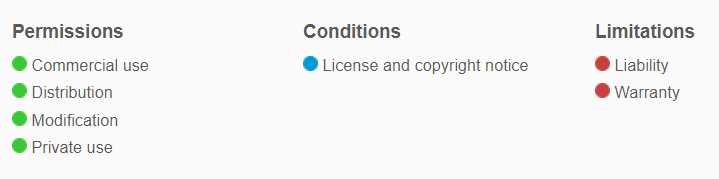
\includegraphics[scale=1]{licenza}
		\centering
		\caption{Punti salienti della licenza MIT}
	\end{figure}
	
	La licenza è visualizzabile nella sua interezza al seguente link:
	\begin{center}
		\url{https://choosealicense.com/licenses/mit/}
	\end{center} 

	\printglossary[style=glossaryStyle, nonumberlist]
	
\end{document}
